\section{Numerical Examples}
\label{section: Chapter4/examples}

In this section, a set of example problems computed with the aforementioned method is presented. These examples illustrate the main capabilities of the approach, but also serve to demonstrate some of the limitations. They all consist of hydrulic fracture propagation in a poroelastic medium. However, different fracture geometries and boundary conditions are explored. The main goal is to ensure that the proposed algorithm works as expected and can handle different scenarios, such as multiple fractures and in-plane crack merging.

Importantly, a true verification procedure is not performed here. For example, mesh convergence studies and comparisons with well-known solutions are yet to be performed. Those require a few enhancements in the solver technology that are currently under development. First, due to the high discrepancy between the scales of degrees of freedom (matrix displacements, fracture apertures and pressures), general purpose linear solvers struggle to converge when the meshes are refined past a certain point. In this case, special preconditioners that take into account the block structure of the system are recommended. CITE SOMEONE. Second, analytical solutions for poroelastic problems are scarce, so, a common verification procedure consists in solving them with vanishing small permeability coefficients to verify convergence towards the KGD solutions (Section XXX) for impermeable media. However, as the permeability decreses, the poromechanics problem starts to display KBB-type instabilities (CITE SOMETHING), which require either modifications to element types or a stabilized formulation, such as (CITE JOSH PAPER). This solver infrastructure enhancements are currently in progress.

For the problems in this Section, the material properties used are listed in Table XX. 

% add table

\subsection{Single fracture under fluid injection with non-homogenous boundary conditions}

In this problem, an initial penny-shaped fracture is injected with a viscous fluid and the boundary conditions are these shown in Figure XXX. Since the boundary conditions are different in the outer faces, the fracture tend to have a prefered propagation direction and therefore, loses its initial circular shape. 

This

% \begin{figure}[h]
%     \centering
%     \begin{subfigure}{.6\textwidth}
%       \centering
%       % This file was created with tikzplotlib v0.10.1.
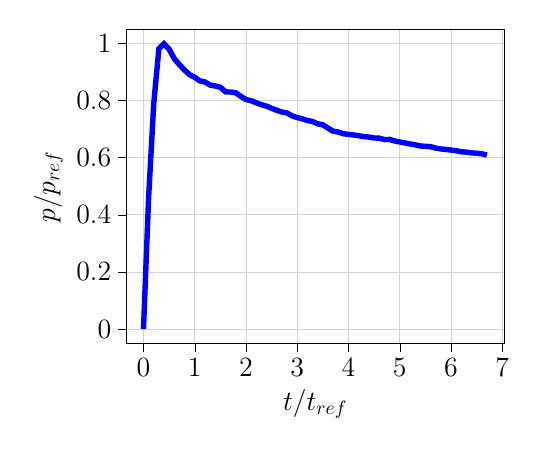
\begin{tikzpicture}[scale=0.7, font=\Large]

\definecolor{lightgray}{RGB}{211,211,211}

\begin{axis}[
tick align=outside,
tick pos=left,
x grid style={lightgray},
xlabel={\(\displaystyle t/t_{ref}\)},
xmajorgrids,
xmin=-0.335, xmax=7.035,
xtick style={color=black},
y grid style={lightgray},
ylabel={\(\displaystyle p/p_{ref}\)},
ymajorgrids,
ymin=-0.0498825329280283, ymax=1.0475331914886,
ytick style={color=black}
]
\addplot [line width=2.8pt, blue]
table {%
0 0
0.1 0.45951217560765
0.2 0.788592266536983
0.3 0.979658043857808
0.4 0.997650658560567
0.5 0.978785067303964
0.6 0.945971757956235
0.7 0.924877167218727
0.8 0.905966129538245
0.9 0.889602759640749
1 0.880357526928354
1.1 0.867671216379265
1.2 0.864233448832077
1.3 0.853114312789821
1.4 0.850108135287821
1.5 0.845620481022948
1.6 0.829505321551291
1.7 0.82892647153026
1.8 0.826514080553166
1.9 0.813655142687903
2 0.802768783688767
2.1 0.798543387344519
2.2 0.791408224631453
2.3 0.784592950157044
2.4 0.779669735090534
2.5 0.771982941261582
2.6 0.764935123584626
2.7 0.759180136109881
2.8 0.755819802453577
2.9 0.745394700232725
3 0.739759343297616
3.1 0.73509236716247
3.2 0.729345702728615
3.3 0.725778734141958
3.4 0.717687645906032
3.5 0.714371573361759
3.6 0.702688940886406
3.7 0.692071117257683
3.8 0.689075788412169
3.9 0.683018346545578
4 0.680940241480926
4.1 0.678761582675207
4.2 0.676155909908243
4.3 0.67303862482668
4.4 0.67141982291266
4.5 0.668213339195578
4.6 0.667744559568312
4.7 0.662721346127251
4.8 0.663129635213632
4.9 0.657892335911165
5 0.654296951897791
5.1 0.650863757765831
5.2 0.647428666367983
5.3 0.644241597549297
5.4 0.640318013987773
5.5 0.638947287170507
5.6 0.638052591816986
5.7 0.632877744620429
5.8 0.629874714646489
5.9 0.62812562862508
6 0.625989632848015
6.1 0.623727478456361
6.2 0.61994558051626
6.3 0.618837276024664
6.4 0.616144894474259
6.5 0.614945973289227
6.6 0.612979236533847
6.7 0.60828213805131
};
\end{axis}

\end{tikzpicture}
%       \caption{}
%       \label{}
%     \end{subfigure}%
%     \begin{subfigure}{.6\textwidth}
%       \centering
%       \input{Chapter4/figures/tikz/mergingFracAperture.tikz}
%       \caption{}
%       \label{}
%     \end{subfigure}%
%       \caption{Lorem Ipsum} 
%       \label{fig:fd}
% \end{figure}

% \begin{figure}[h]
%     \centering
%     \begin{subfigure}{.6\textwidth}
%       \centering
%       % This file was created with tikzplotlib v0.10.1.
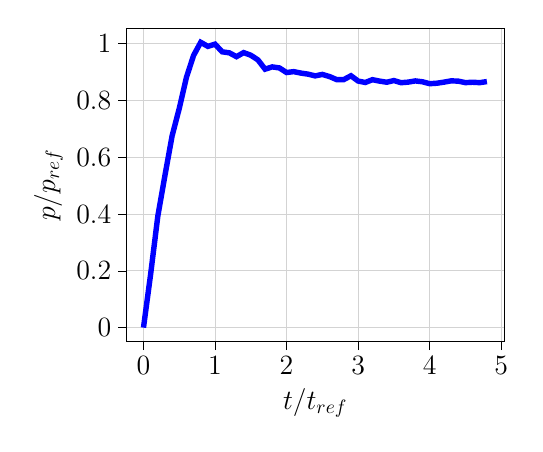
\begin{tikzpicture}[scale=0.7, font=\Large]

\definecolor{lightgray}{RGB}{211,211,211}

\begin{axis}[
tick align=outside,
tick pos=left,
x grid style={lightgray},
xlabel={\(\displaystyle t/t_{ref}\)},
xmajorgrids,
xmin=-0.24, xmax=5.04,
xtick style={color=black},
y grid style={lightgray},
ylabel={\(\displaystyle p/p_{ref}\)},
ymajorgrids,
ymin=-0.0502281761912294, ymax=1.05479170001582,
ytick style={color=black}
]
\addplot [line width=2.8pt, blue]
table {%
0 0
0.1 0.188445766752718
0.2 0.391947508110223
0.3 0.535895204930158
0.4 0.675176372415468
0.5 0.771710290038251
0.6 0.880899367078848
0.7 0.958412412909037
0.8 1.00456352382459
0.9 0.990324948221893
1 0.998054606057314
1.1 0.971102817197564
1.2 0.967556258546069
1.3 0.954084839144053
1.4 0.968359167181806
1.5 0.959116405852193
1.6 0.942617944583139
1.7 0.910026091662552
1.8 0.918049400613525
1.9 0.914348525898006
2 0.898192078875057
2.1 0.901362856789026
2.2 0.896214438996315
2.3 0.892511564645737
2.4 0.886358846124087
2.5 0.891502924804546
2.6 0.884023936770732
2.7 0.873345919605794
2.8 0.873412882862689
2.9 0.886829564180904
3 0.868198311002277
3.1 0.863129333961807
3.2 0.873000347785484
3.3 0.867964509851173
3.4 0.864042793812506
3.5 0.869939165930708
3.6 0.862387111210862
3.7 0.864402846886308
3.8 0.868605632794512
3.9 0.865597652226709
4 0.8589197342603
4.1 0.860522133055493
4.2 0.864358319941601
4.3 0.868875836425173
4.4 0.867843224744737
4.5 0.862641238764823
4.6 0.863963070087864
4.7 0.862565672752955
4.8 0.866328855022948
};
\end{axis}

\end{tikzpicture}

%       \caption{}
%       \label{}
%     \end{subfigure}%
%     \begin{subfigure}{.6\textwidth}
%       \centering
%       % This file was created with tikzplotlib v0.10.1.
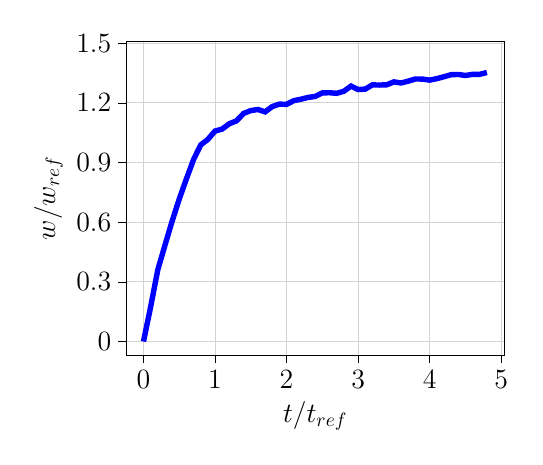
\begin{tikzpicture}[scale=0.7, font=\Large]

\definecolor{lightgray}{RGB}{211,211,211}

\begin{axis}[
tick align=outside,
tick pos=left,
x grid style={lightgray},
xlabel={\(\displaystyle t/t_{ref}\)},
xmajorgrids,
xmin=-0.24, xmax=5.04,
xtick style={color=black},
y grid style={lightgray},
ytick distance=0.3,
ylabel={\(\displaystyle w/w_{ref}\)},
ymajorgrids,
ymin=-0.0676150128188689, ymax=1.51,
ytick style={color=black}
]
\addplot [line width=2.8pt, blue]
table {%
0 0
0.1 0.174099460537345
0.2 0.36037093622801
0.3 0.483736302329922
0.4 0.604657400483929
0.5 0.71627362525909
0.6 0.817741763252065
0.7 0.914673087058184
0.8 0.988043835003288
0.9 1.01615749619579
1 1.05781999647227
1.1 1.06795558571426
1.2 1.09487671410362
1.3 1.10903211791217
1.4 1.14665606861212
1.5 1.16093104459679
1.6 1.16625499737314
1.7 1.15430886393875
1.8 1.18121700420342
1.9 1.19330912726223
2 1.19206895215774
2.1 1.21057291458408
2.2 1.21798236109138
2.3 1.22691783387849
2.4 1.23188777939765
2.5 1.24970648339836
2.6 1.25053556512246
2.7 1.24766343959738
2.8 1.2578584515492
2.9 1.28381515930564
3 1.26659534216305
3.1 1.26894556444263
3.2 1.29005564497642
3.3 1.28918001813621
3.4 1.29050708947248
3.5 1.30520754884353
3.6 1.29951568143079
3.7 1.30872862561227
3.8 1.31974418932991
3.9 1.31922767023963
4 1.31398053120865
4.1 1.32143831069796
4.2 1.33095372857038
4.3 1.34126355648886
4.4 1.34234868328863
4.5 1.33716954069027
4.6 1.34310704227726
4.7 1.34310814299716
4.8 1.35230025637738
};
\end{axis}

\end{tikzpicture}

%       \caption{}
%       \label{}
%     \end{subfigure}%
%       \caption{Lorem Ipsum} 
%       \label{fig:fd}
% \end{figure}

\noindent% This file was created with tikzplotlib v0.10.1.
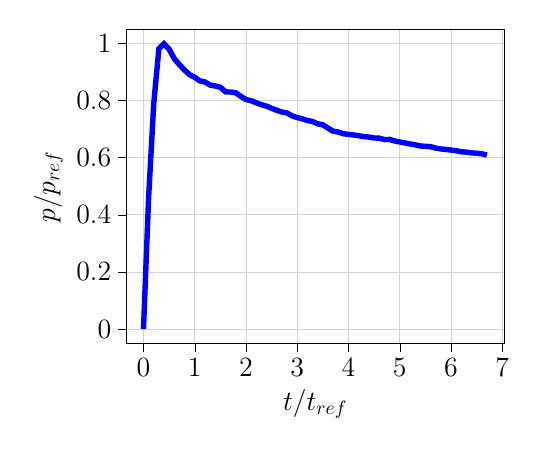
\begin{tikzpicture}[scale=0.7, font=\Large]

\definecolor{lightgray}{RGB}{211,211,211}

\begin{axis}[
tick align=outside,
tick pos=left,
x grid style={lightgray},
xlabel={\(\displaystyle t/t_{ref}\)},
xmajorgrids,
xmin=-0.335, xmax=7.035,
xtick style={color=black},
y grid style={lightgray},
ylabel={\(\displaystyle p/p_{ref}\)},
ymajorgrids,
ymin=-0.0498825329280283, ymax=1.0475331914886,
ytick style={color=black}
]
\addplot [line width=2.8pt, blue]
table {%
0 0
0.1 0.45951217560765
0.2 0.788592266536983
0.3 0.979658043857808
0.4 0.997650658560567
0.5 0.978785067303964
0.6 0.945971757956235
0.7 0.924877167218727
0.8 0.905966129538245
0.9 0.889602759640749
1 0.880357526928354
1.1 0.867671216379265
1.2 0.864233448832077
1.3 0.853114312789821
1.4 0.850108135287821
1.5 0.845620481022948
1.6 0.829505321551291
1.7 0.82892647153026
1.8 0.826514080553166
1.9 0.813655142687903
2 0.802768783688767
2.1 0.798543387344519
2.2 0.791408224631453
2.3 0.784592950157044
2.4 0.779669735090534
2.5 0.771982941261582
2.6 0.764935123584626
2.7 0.759180136109881
2.8 0.755819802453577
2.9 0.745394700232725
3 0.739759343297616
3.1 0.73509236716247
3.2 0.729345702728615
3.3 0.725778734141958
3.4 0.717687645906032
3.5 0.714371573361759
3.6 0.702688940886406
3.7 0.692071117257683
3.8 0.689075788412169
3.9 0.683018346545578
4 0.680940241480926
4.1 0.678761582675207
4.2 0.676155909908243
4.3 0.67303862482668
4.4 0.67141982291266
4.5 0.668213339195578
4.6 0.667744559568312
4.7 0.662721346127251
4.8 0.663129635213632
4.9 0.657892335911165
5 0.654296951897791
5.1 0.650863757765831
5.2 0.647428666367983
5.3 0.644241597549297
5.4 0.640318013987773
5.5 0.638947287170507
5.6 0.638052591816986
5.7 0.632877744620429
5.8 0.629874714646489
5.9 0.62812562862508
6 0.625989632848015
6.1 0.623727478456361
6.2 0.61994558051626
6.3 0.618837276024664
6.4 0.616144894474259
6.5 0.614945973289227
6.6 0.612979236533847
6.7 0.60828213805131
};
\end{axis}

\end{tikzpicture}
\hspace{0.5cm}
\input{Chapter4/figures/tikz/mergingFracAperture.tikz}

\noindent% This file was created with tikzplotlib v0.10.1.
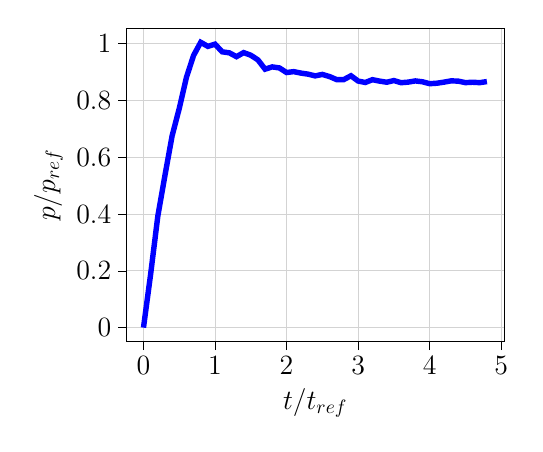
\begin{tikzpicture}[scale=0.7, font=\Large]

\definecolor{lightgray}{RGB}{211,211,211}

\begin{axis}[
tick align=outside,
tick pos=left,
x grid style={lightgray},
xlabel={\(\displaystyle t/t_{ref}\)},
xmajorgrids,
xmin=-0.24, xmax=5.04,
xtick style={color=black},
y grid style={lightgray},
ylabel={\(\displaystyle p/p_{ref}\)},
ymajorgrids,
ymin=-0.0502281761912294, ymax=1.05479170001582,
ytick style={color=black}
]
\addplot [line width=2.8pt, blue]
table {%
0 0
0.1 0.188445766752718
0.2 0.391947508110223
0.3 0.535895204930158
0.4 0.675176372415468
0.5 0.771710290038251
0.6 0.880899367078848
0.7 0.958412412909037
0.8 1.00456352382459
0.9 0.990324948221893
1 0.998054606057314
1.1 0.971102817197564
1.2 0.967556258546069
1.3 0.954084839144053
1.4 0.968359167181806
1.5 0.959116405852193
1.6 0.942617944583139
1.7 0.910026091662552
1.8 0.918049400613525
1.9 0.914348525898006
2 0.898192078875057
2.1 0.901362856789026
2.2 0.896214438996315
2.3 0.892511564645737
2.4 0.886358846124087
2.5 0.891502924804546
2.6 0.884023936770732
2.7 0.873345919605794
2.8 0.873412882862689
2.9 0.886829564180904
3 0.868198311002277
3.1 0.863129333961807
3.2 0.873000347785484
3.3 0.867964509851173
3.4 0.864042793812506
3.5 0.869939165930708
3.6 0.862387111210862
3.7 0.864402846886308
3.8 0.868605632794512
3.9 0.865597652226709
4 0.8589197342603
4.1 0.860522133055493
4.2 0.864358319941601
4.3 0.868875836425173
4.4 0.867843224744737
4.5 0.862641238764823
4.6 0.863963070087864
4.7 0.862565672752955
4.8 0.866328855022948
};
\end{axis}

\end{tikzpicture}

\hspace{0.5cm}
% This file was created with tikzplotlib v0.10.1.
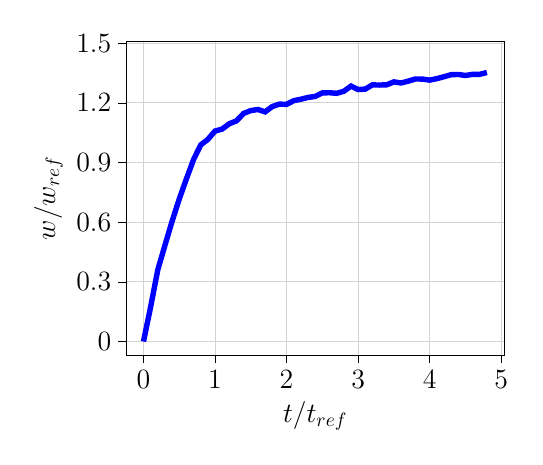
\begin{tikzpicture}[scale=0.7, font=\Large]

\definecolor{lightgray}{RGB}{211,211,211}

\begin{axis}[
tick align=outside,
tick pos=left,
x grid style={lightgray},
xlabel={\(\displaystyle t/t_{ref}\)},
xmajorgrids,
xmin=-0.24, xmax=5.04,
xtick style={color=black},
y grid style={lightgray},
ytick distance=0.3,
ylabel={\(\displaystyle w/w_{ref}\)},
ymajorgrids,
ymin=-0.0676150128188689, ymax=1.51,
ytick style={color=black}
]
\addplot [line width=2.8pt, blue]
table {%
0 0
0.1 0.174099460537345
0.2 0.36037093622801
0.3 0.483736302329922
0.4 0.604657400483929
0.5 0.71627362525909
0.6 0.817741763252065
0.7 0.914673087058184
0.8 0.988043835003288
0.9 1.01615749619579
1 1.05781999647227
1.1 1.06795558571426
1.2 1.09487671410362
1.3 1.10903211791217
1.4 1.14665606861212
1.5 1.16093104459679
1.6 1.16625499737314
1.7 1.15430886393875
1.8 1.18121700420342
1.9 1.19330912726223
2 1.19206895215774
2.1 1.21057291458408
2.2 1.21798236109138
2.3 1.22691783387849
2.4 1.23188777939765
2.5 1.24970648339836
2.6 1.25053556512246
2.7 1.24766343959738
2.8 1.2578584515492
2.9 1.28381515930564
3 1.26659534216305
3.1 1.26894556444263
3.2 1.29005564497642
3.3 1.28918001813621
3.4 1.29050708947248
3.5 1.30520754884353
3.6 1.29951568143079
3.7 1.30872862561227
3.8 1.31974418932991
3.9 1.31922767023963
4 1.31398053120865
4.1 1.32143831069796
4.2 1.33095372857038
4.3 1.34126355648886
4.4 1.34234868328863
4.5 1.33716954069027
4.6 1.34310704227726
4.7 1.34310814299716
4.8 1.35230025637738
};
\end{axis}

\end{tikzpicture}

